\section{Results}
\label{sec:results}
In this section, we will show and discuss some of the results of the research described in the earlier sections. More specifically: we show how exactly the popularity of various topics changed over time. Since we have a thousand topics, we cannot show charts for every individual topic. Instead, we picked a few topics we consider to be interesting and show these. 
% TODO: uncomment if we want to show this.
%For a full list, we refer to a webpage where we published all our data which has interactive charts\footnote{\url{http://bcleenders.github.io/AIM/}}.

% TODO: do we want to keep this one? IMHO it doesn't add much... (but maybe I'm missing the point)
%\begin{figure}[H]
%	\caption{Topic group sizes}
%	\label{fig:topicsizes}
%	\centering
%	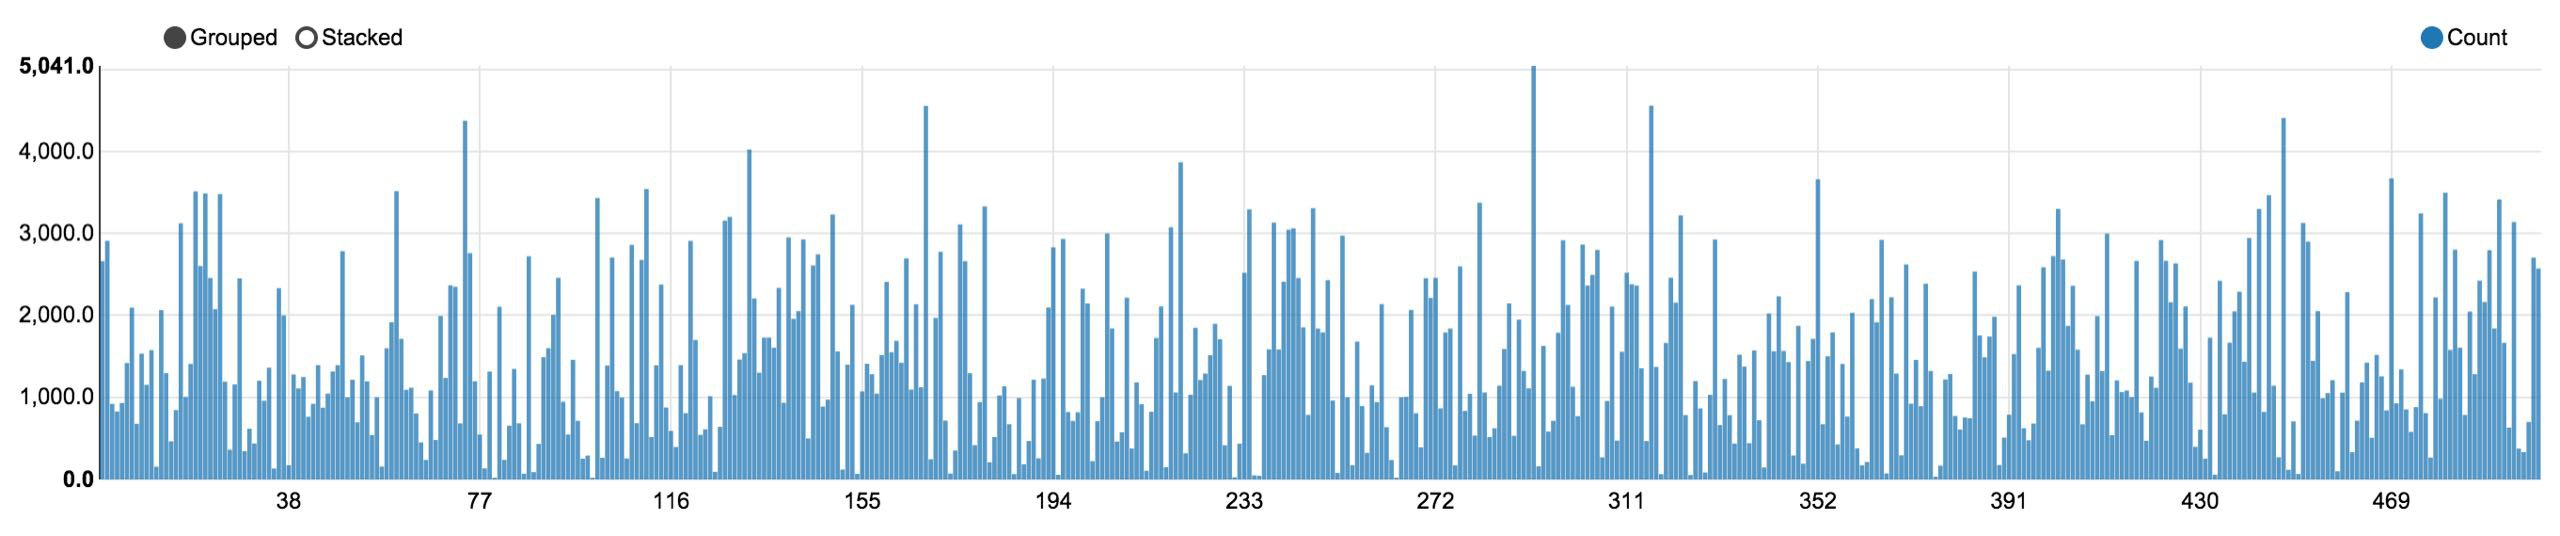
\includegraphics[width=14cm]{topicsizes}
%\end{figure}

Note that, since there are 1,000 topics, the average popularity is 10 basis points (10\textpertenthousand). The popularity is positively skewed, however: roughly a third of the months/topic combinations have a popularity below 1\textpertenthousand. To stress this point, we include figure~\ref{fig:popularitydistribution}.

\begin{figure}[H]
	\caption{Popularity distribution - popularity (in bp) vs. number of topic/months}
	\label{fig:popularitydistribution}
	\centering
	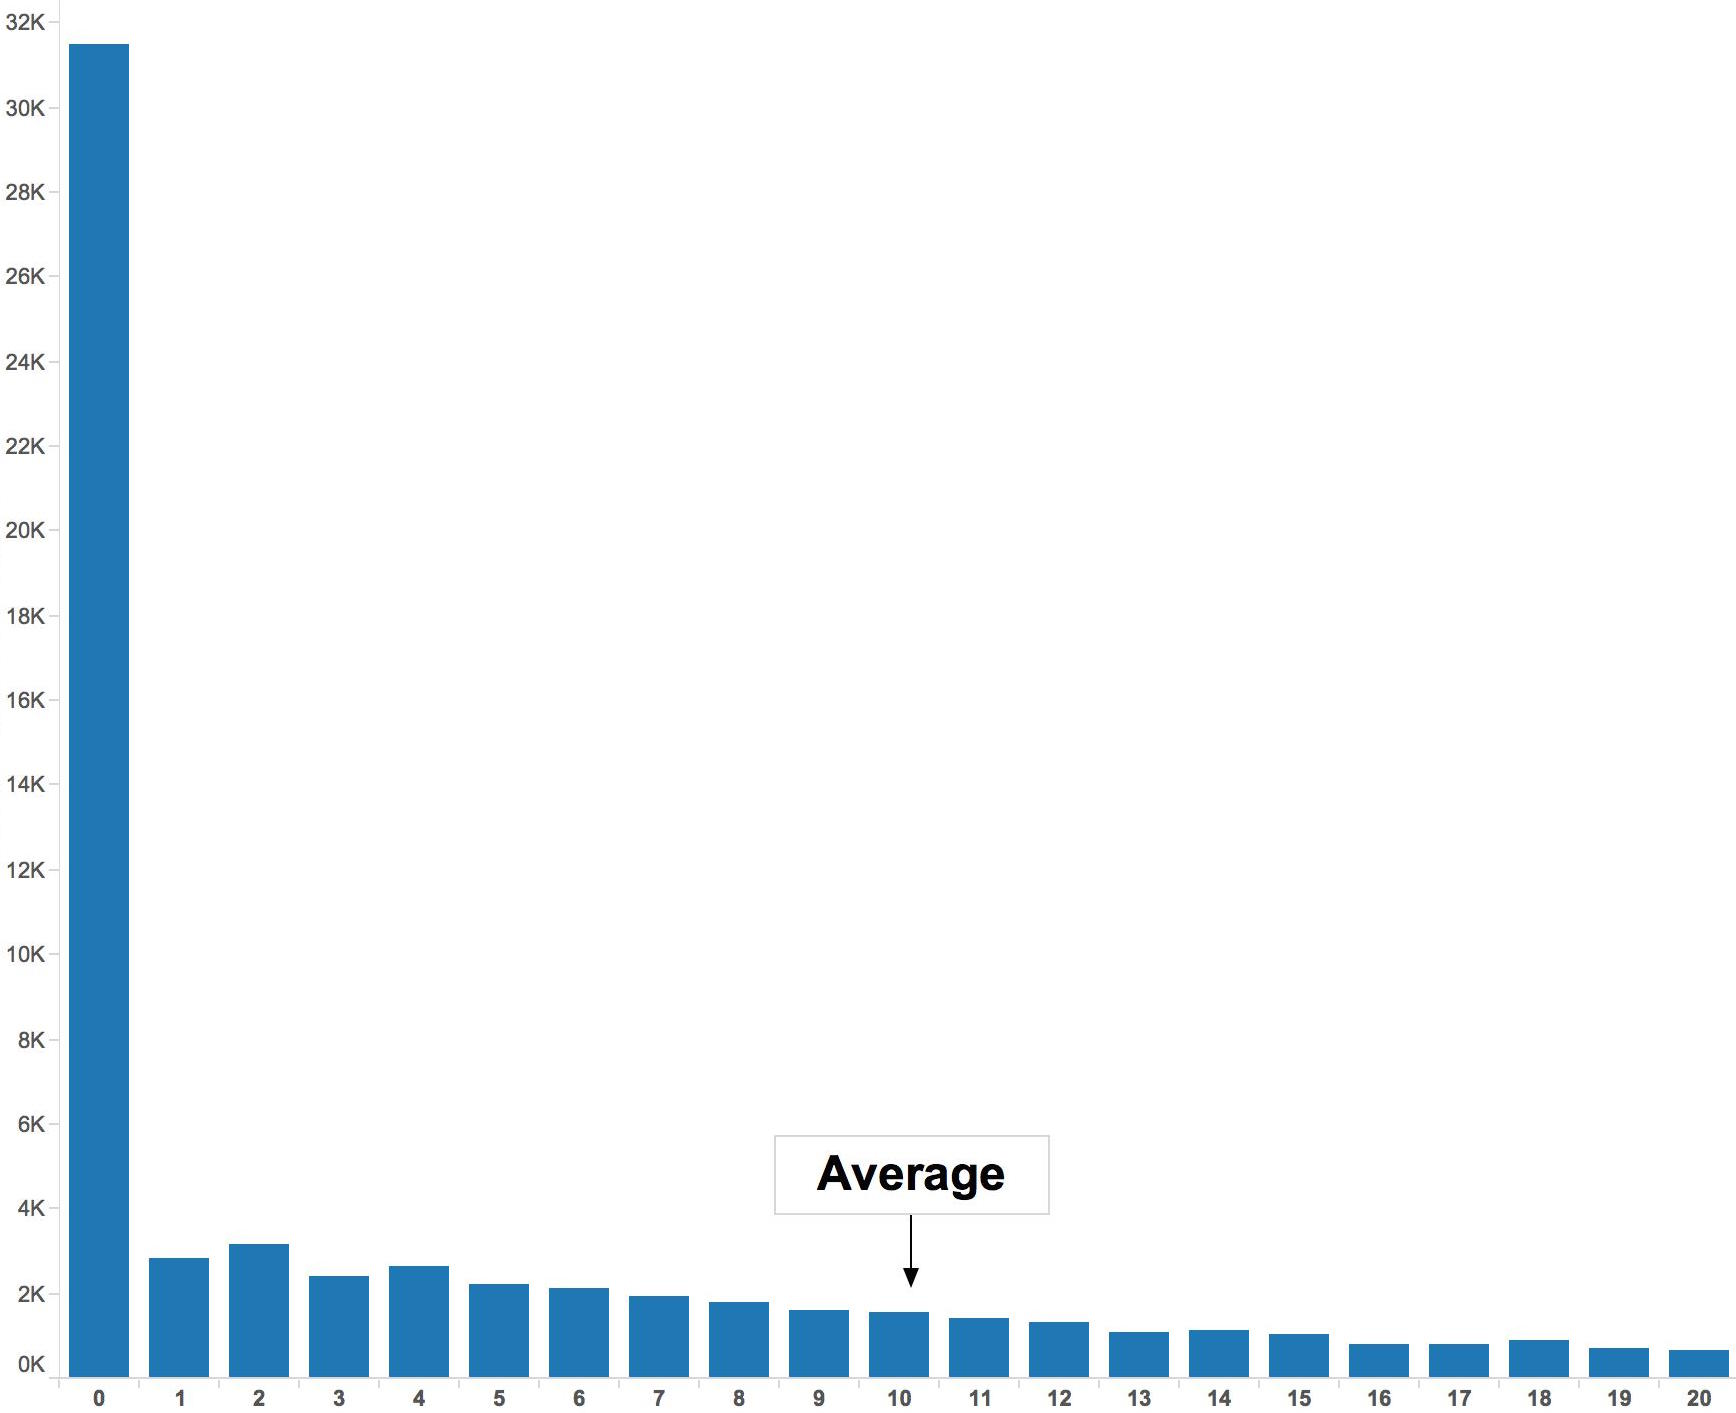
\includegraphics[width=8cm]{popularity_distribution_basispoints_buckets}
\end{figure}

\subsection{Popularity plots}
In this section, we will show some awesome plots of how the popularity of various topics changed over time.

\begin{figure}[H] % Topic 412
	\caption{Popularity of Docker, CoreOS, etcd, containers, OpenStack}
	\label{fig:trend_docker}
	\centering
	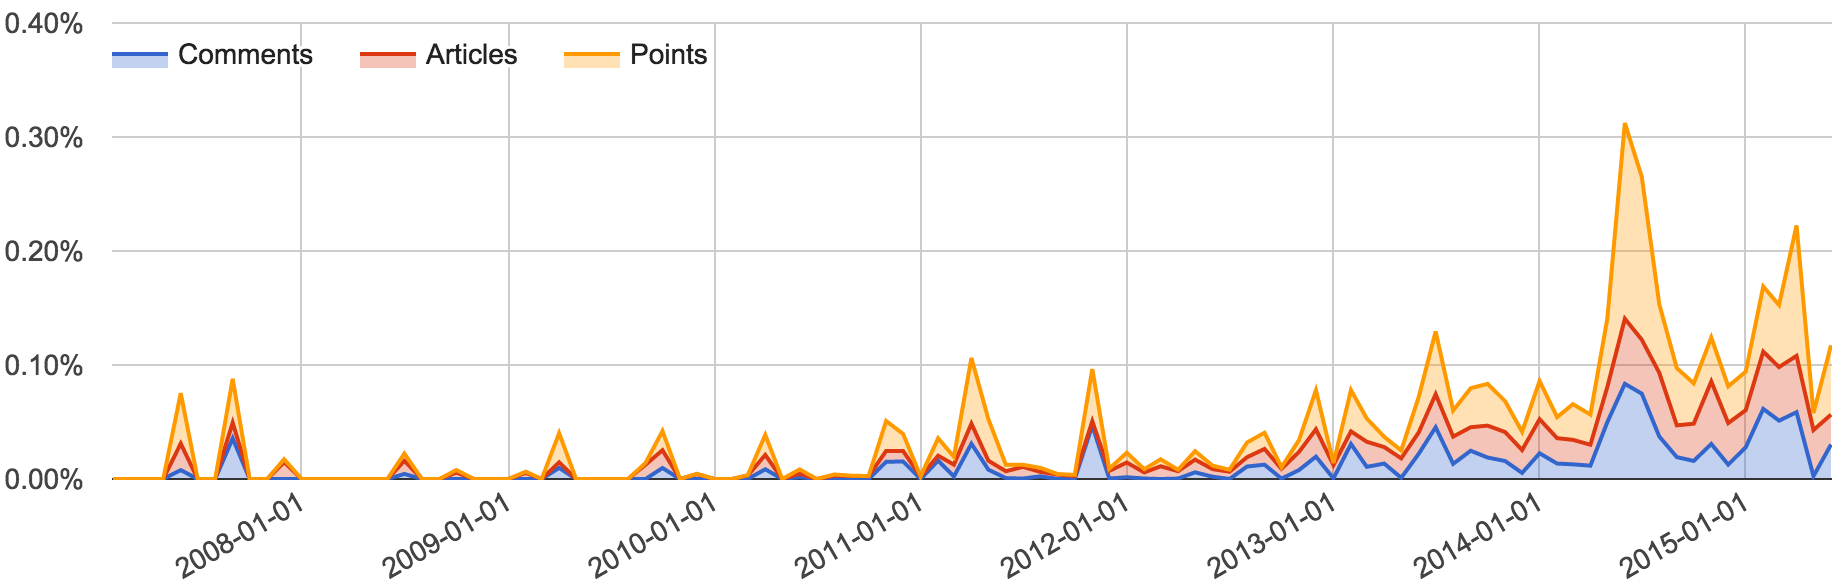
\includegraphics[width=14cm]{topic_trends/docker_relative}
	% docker coreos etcd images:containers openshift mesos deis openstack orchestration dokku
\end{figure}
We start the overview with a trend plot (figure~\ref{fig:trend_docker}) of a new and upcoming technique: containerization. Docker and CoreOS were released in 2014 and before that, containerization was already used as a term for seperating Linux processes (which explains earlier peaks). The trends show how the release of Docker 1.0 (June 2014) created a lot of buzz, and the sustained popularity afterwards.

\begin{figure}[H] % Topic 383
	\caption{Popularity of Elon Musk, SpaceX, Tesla, Hyperloop}
	\label{fig:trend_elon}
	\centering
	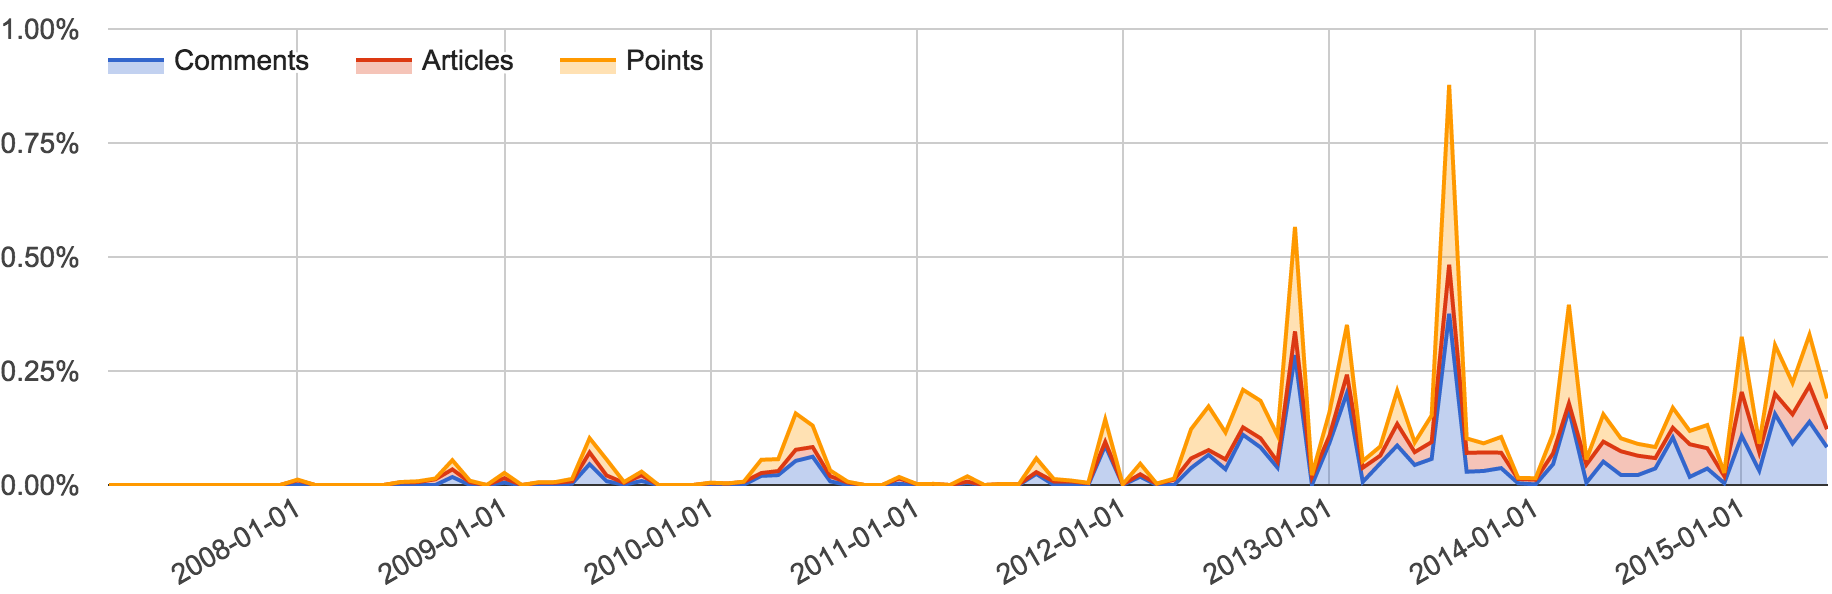
\includegraphics[width=14cm]{topic_trends/elon_relative}
	% elon musks spacex musk's tesla hyperloop test track musk
\end{figure}
Elon Musk is described by Wired.com as a ''maverick entrepreneur" due to his big and risky projects. We see this reflected in the chart of his popularity (figure~\ref{fig:trend_elon}). Halfway 2010, Elon was out of cash (despite a 200 million dollar buyout from PayPal), which sparked some interest. The big spike late 2012 marks his expressed intent to have SpaceX (his spacecraft company) fly to Mars. The biggest spike in the chart, halfway 2013, marks the introduction of Hyperloop, a high-speed transportation system.

\begin{figure}[H] % Topic 79
	\caption{Popularity of keynote, Apple, @scale, developers conference}
	\label{fig:trend_keynote}
	\centering
	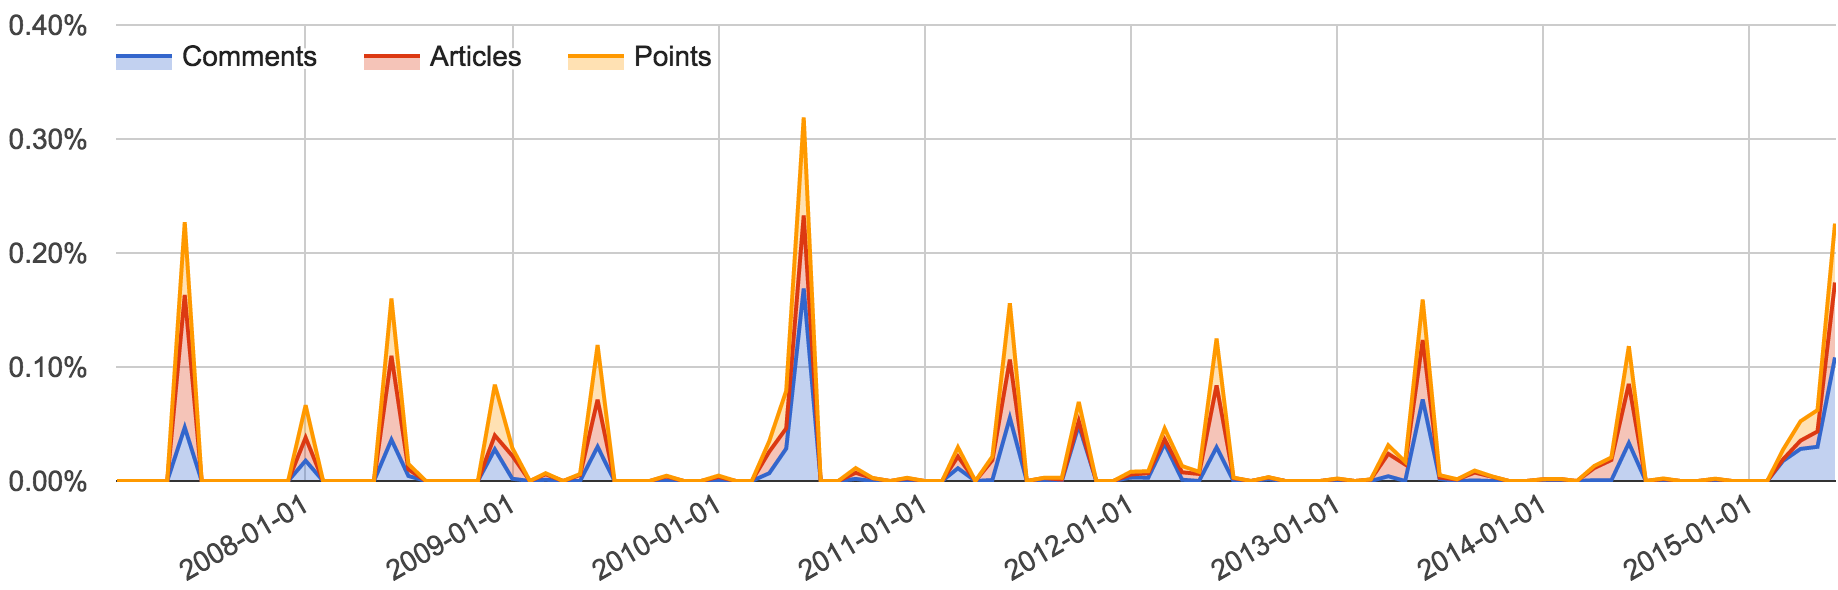
\includegraphics[width=14cm]{topic_trends/keynote_relative}
	% keynote apple live yesterday's apple's @scale apple developers conference keynotes conference macworld
\end{figure}
In the popularity charts of keynote-related topics (figure~\ref{fig:trend_keynote}), one can see yearly patterns of spiking popularity. Each June has a spike of over 0.1\%, which corresponds to Apple's annual WWDC (Worldwide Developers Conference). The spikes smaller than 0.1\% are just noise.

\begin{figure}[H] % Topic 579
	\caption{Popularity of Steve Jobs, Wozniak, imagineers}
	\label{fig:trend_jobs}
	\centering
	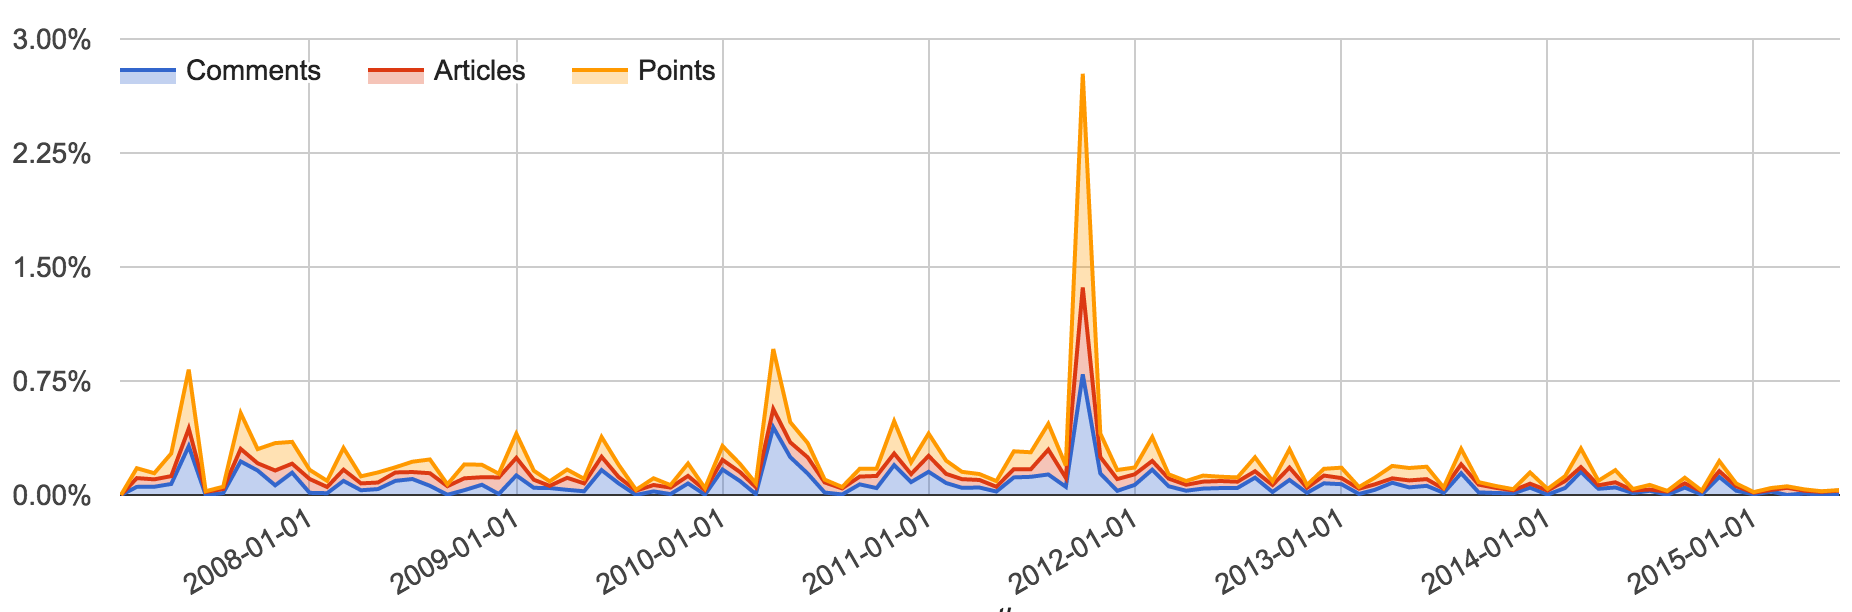
\includegraphics[width=14cm]{topic_trends/jobs_relative}
	% jobs wozniak woz jobs. steve steves jobs's jobssteve imagineers wozs
	% Interesting: Tim Cook is not in this cluster, and his coming out is therefore not visible in this graph
\end{figure}

On the topic of Apple: not only it's products spark the interest of the Hacker News community; it's former CEO also had a big impact in the community. We show figure~\ref{fig:trend_jobs} to indicate the enormous impact the death of Steve Jobs had. He shares this topic group with his co-founder Steve Wozniak, but the news of his death (October 5th, 2011) dwarfs all other events in Hacker News history.

\begin{figure}[H] % Topic 17
	\caption{Popularity of Raspberry Pi, Kindleberry}
	\label{fig:trend_raspberry}
	\centering
	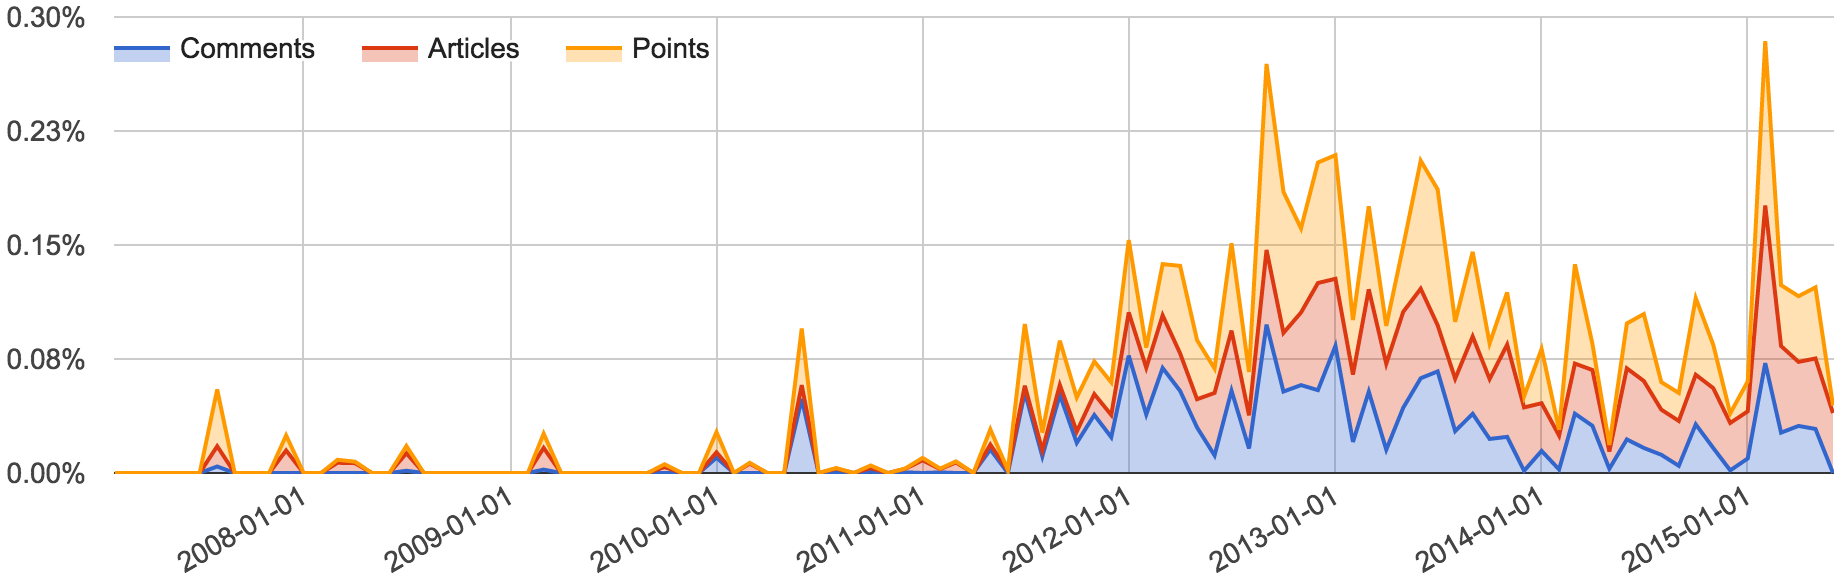
\includegraphics[width=14cm]{topic_trends/raspberry_relative}
	% raspberry pi's kindleberry pis navio+ motherbone-tm-pione-tm- piface razberry rpi raspberrypi
\end{figure}

\begin{figure}[H] % Topic 70
	\caption{Popularity of Edward Snowden, Wistleblower, leaks, Reddit}
	\label{fig:trend_snowden}
	\centering
	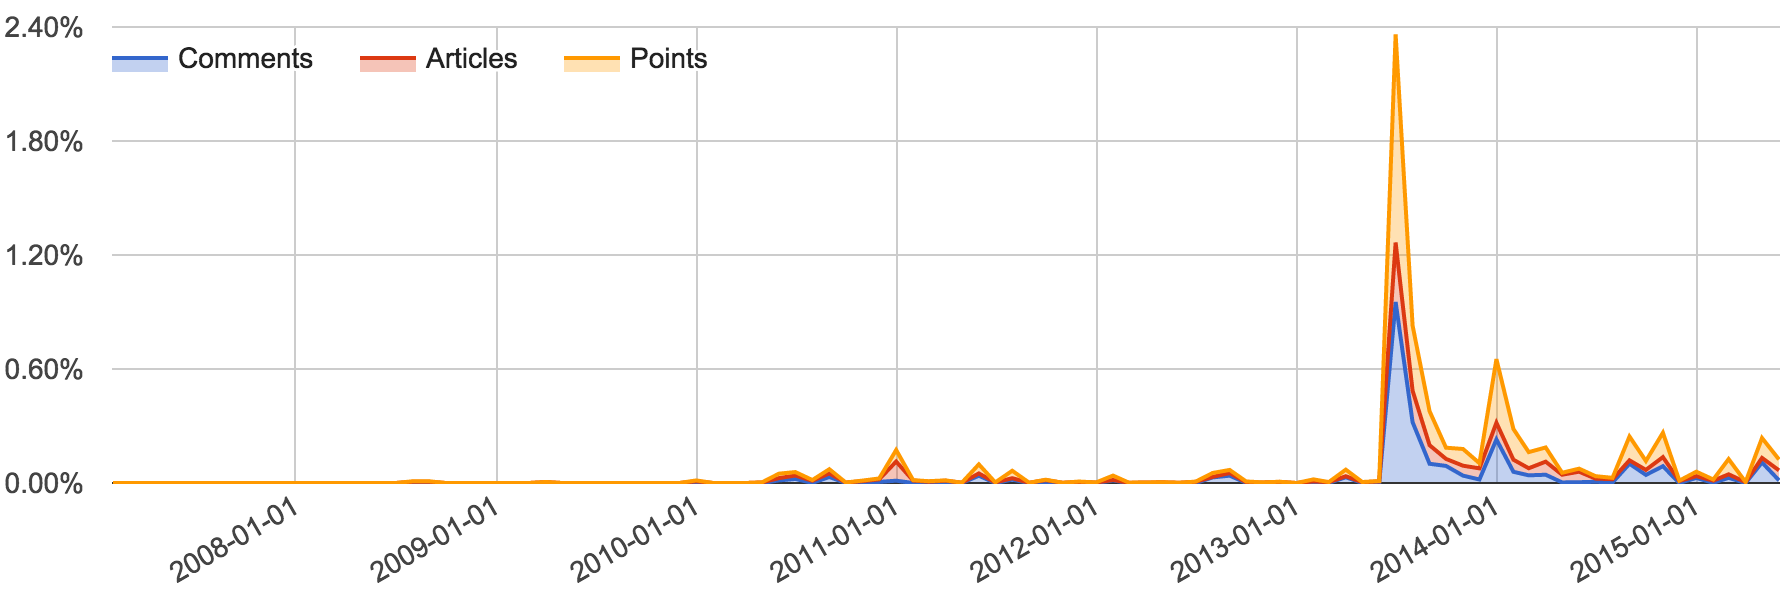
\includegraphics[width=14cm]{topic_trends/snowden_relative}
	% edward whistleblower contractor-turned-whistleblower snowden.the snowden's leaker snowdens reddit.comsubmitted snowden. snowden.in
\end{figure}
\lipsum[1]
